\documentclass[leqno]{article}
\usepackage{graphicx}
%% following is added by imaxima output
\usepackage{verbatim}
\usepackage[cmbase]{flexisym}
\usepackage{bbold}
%bbold above conflicts with amssymb \usepackage{amssymb}
\usepackage{breqn}
\setkeys{breqn}{compact}

%\usepackage{amssymb} this breaks bbold numeral
%\usepackage{amsmath}



\setlength{\textwidth}{180mm}
\setlength{\oddsidemargin}{15mm}
\addtolength{\oddsidemargin}{-1in}
\setlength{\evensidemargin}{15mm}
\addtolength{\evensidemargin}{-1in}

\newcommand{\ifrac}[2]{\frac{#1}{#2}}
\newcommand{\ifracd}[2]{\frac{#1}{#2}}
\newcommand{\ifracn}[2]{\frac{#1}{#2}}
\newcommand{\isubscript}[2]{{#1}_{#2}}
\newcommand{\iexpt}[2]{{#1}^{#2}}
\newcommand{\isqrt}[1]{\sqrt{#1}}
%% end lines added by imaxima output

\newcommand{\ket}[1]{{\lvert#1 \rangle}}
\newcommand{\bra}[1]{{\langle#1 \rvert}}
\newcommand{\func}[2]{{\bf #1}($#2$)}
\newcommand{\marray}[2]{{\bf #1}[$#2$]}
\newcommand{\fs}[1]{{\bf #1}}
\newcommand{\farg}[1]{{\it #1}}
\newcommand{\op}[1]{{\bf #1}}
\newcommand{\maxcom}{\textsuperscript{$\dagger$}}

\begin{document}


\title{Quantum Information Package For The Maxima Computer
  Algebra System}
\author{G. John Lapeyre, Jr.}

\maketitle

\begin{verbatim}
         Copyright (c)  2008  Gerald John Lapeyre Jr.
         Permission is granted to copy, distribute and/or modify this document
         under the terms of the GNU Free Documentation License, Version 1.2
         or any later version published by the Free Software Foundation;
         with no Invariant Sections, no Front-Cover Texts, and no Back-Cover Texts.
         A copy of the license is included in the distribution of the source
         code of the software accompanying this manual in the file fdl.txt.
\end{verbatim}

\section{Introduction}

This quantum information package for the Maxima computer
algebra system allows the manipulation of instances of objects,
operators,vectors,tensors, {\it etc.}  appearing in quantum
information theory.  More precisely these objects are
typically represented in a particular basis as row and column vectors
and matrices, whose entries may be explicit numbers (of
various classes) or algebraic expressions. This document
describes the functions and data in the package and how to
use them with Maxima, assuming that you do not know much
about Maxima, but do know quantum information theory.

Examples of the facilities of the
package are
\begin{itemize}
  \begin{item}
    Methods for constructing pure and mixed states and operators.
  \end{item}
  \begin{item}
    Methods for executing standard operations found in
    computational linear algebra as well as the tensor
    product, partial trace, etc.
  \end{item}
  \begin{item}
    Functions to compute commonly appearing quantities such as entropy and purity.
  \end{item}
\end{itemize}

Some suggestions and things to be aware of in the following sections.
\begin{itemize}
  \begin{item}
    You probably need to read at least a ten minute tutorial before or in conjunction
    with reading this document. There are several listed at the Maxima website, and
    others that a search engine can find. If you are too impatient there is a very
    brief introduction to Maxima below.
  \end{item}
  \begin{item}
    Functions and features that are part of the standard Maxima distribution,
    rather than part of the quantum information
    package are marked, where not obvious, with the dagger superscript--- \maxcom.
  \end{item}
  \begin{item}
    There are several user interfaces to the Maxima. All the
    examples here are generated using the imaxima package
    for the emacs editor/environment, but the results are
    similar to other graphical frontends to Maxima.
  \end{item}
  \begin{item}
    Most functions currently work only with qubits, others for variable number of
    states.
  \end{item}
\end{itemize}

The package is intended to be used for research in the theory of entanglement
and quantum information and related fields. 

\subsection{Acknowledgments}

Some of the ideas used in this package are inspired by the package qdens
written for a proprietary symbolic algebra system. (put reference here)

\section{Tutorial introduction}

The majority of the examples below are taken from the regression tests for
the qinf package or from the author's research.

The package is loaded by entering the command
%\verb|load("qinf.mac");|.
\texttt{load("qinf.mac");}
\begin{verbatim}
(%i2) load("qinf.mac")
\end{verbatim}
\begin{dmath}[number={\%o4}]
 \verb|qinf.mac|\end{dmath}


\subsection{Using Maxima}
There are several tutorials and manuals available for Maxima. Here is a very brief one
focused on aiding the introduction to the qinf package.

We will not give examples of matrices until later,
but point out that the notation for matrix multiplication in
Maxima is a dot, eg. \verb|A . B|. If $A$ is a $m\times n$
and $B$ a $p\times q$ matrix, then the result is a $n\times
p$ matrix. The inner product of quantum state vectors, the
outer product of quantum state vectors, the composition of
operators, and the mapping of one vector to another by an
operator are all special cases of matrix multiplication and
are all represented by the dot.

Maxima can use exact real and complex numbers or the
standard floating point approximations, or arbitrary
precision floating point numbers.  Numerical expressions are
simplified upon entry. Each input line must be terminated by
a semicolon (some interfaces do this automatically) or by a
dollar sign, which suppresses the output.
\begin{verbatim}
(%i1) 1 + 1;
\end{verbatim}
\begin{dmath}[number={\%o1}]
  2\end{dmath} 
For example, \verb| a : b+c ;| evaluates \verb|b+c| and assigns the result to \verb|a|.
On the other hand \verb| a(x,y) := x^y ;| defines the function $a(x,y)$.
\begin{verbatim}
(%i2) a : 2 * 2;
\end{verbatim}
\begin{dmath}[number={\%o2}]
 4\end{dmath}
\begin{verbatim}
(%i3) a;
\end{verbatim}
\begin{dmath}[number={\%o3}]
 4\end{dmath}
\begin{verbatim}
(%i4) b : expand( (x+y)^4 );
\end{verbatim}
\begin{dmath}[number={\%o4}]
 y^{4}+4\*x\*y^{3}+6\*x^{2}\*y^{2}+4\*x^{3}\*y+x^{4}\end{dmath}
 Suppress the output here, because it's big-- $51$ terms.
\begin{verbatim}
(%i5) b : expand( (x+y)^50 )$
(%i6) length(b);
\end{verbatim}
\begin{dmath}[number={\%o6}]
 51\end{dmath}
Exact numbers and floating point approximations.
\begin{verbatim}
(%i7)  1  + sqrt(2);
\end{verbatim}
\begin{dmath}[number={\%o7}]
 \isqrt{2}+1\end{dmath}
\begin{verbatim}
(%i8)  1  + sqrt(2), float;
\end{verbatim}
\begin{dmath}[number={\%o8}]
 2.4142135623730949\end{dmath}
Defining and using a function.
\begin{verbatim}
(%i9) f(x) := 3 * cos(x);
\end{verbatim}
\begin{dmath}[number={\%o9}]
 f\left(x\right):=3\*\cos x\end{dmath}
\begin{verbatim}
(%i10) f(a);
\end{verbatim}
\begin{dmath}[number={\%o10}]
 3\*\cos 4\end{dmath}
\begin{verbatim}
(%i11) f(0);
\end{verbatim}
\begin{dmath}[number={\%o11}]
 3\end{dmath}
Complex numbers.
\begin{verbatim}
(%i12) expand ( (1 + 2 * %i)^2 );
\end{verbatim}
\begin{dmath}[number={\%o12}]
 4\*i-3\end{dmath}
Special numbers.
\begin{verbatim}
(%i13) cos(%pi/2);
\end{verbatim}
\begin{dmath}[number={\%o13}]
 0\end{dmath}
\begin{verbatim}
(%i14) %e^(%i * %pi/2);
\end{verbatim}
\begin{dmath}[number={\%o14}]
 i\end{dmath}

\subsection{Creating and manipulating states and operators}

\subsubsection{Representation of states and operators}
Kets are represented by $n \times 1$ matrices, bras by $1
\times n$ matrices. These vectors are in the $z$ basis.
Bras and kets representing the same
states are related by the conjugate transpose function.
Density operators and other operators are represented by
matrices. The tensor product is represented by the Kronecker
product. There is no strong typing. You are responsible
for knowing that a particular vector represents a state vector
in the appropriate space. That is, there is no facility to 
distinguish between a vector in the product space of 
two qubits ${\cal H}_1 \otimes {\cal H}_2 $ and the space of
a single four state qudit.

\subsection{Creating instances of states}
Here are some methods for creating instances of states, from scratch or
from other states. Although all operators  `create' states in this
sense, we omit most of them here, because they are better described as manipulating
states.

%\subsubsection{\func{ket}{i_1,i_2,\ldots,i_n},\func{bra}{i_1,i_2,\ldots,i_n}}
%\fs{ket} and \fs{bra} return $n$-partite states.

\subsubsection{\func{ketz}{i_1,\ldots,i_n}, \func{braz}{i_1,\ldots,i_n},
\func{ketx}{i_1,\ldots,i_n}, \func{brax}{i_1,\ldots,i_n},
  \func{kety}{i_1,\ldots,i_n}, \func{bray}{i_1,\ldots,i_n}}
 
create normalized $n$-partite statesin the z-basis. In all cases
$i_n$ are $0$ or $1$. The pair \fs{ketz} and \fs{braz} produce
eigenstates of $\sigma_z^{(1)} \otimes \cdots \otimes \sigma_z^{(n)}$,
with the index $i=0$ selecting the state with eigenvalue $1$ and
$i=1$ selecting the state with eigenvalue $-1$.
In other words the ket produced represents $\ket{i_1,i_2,\ldots,i_n}.$
\begin{verbatim}
(%i3) ketz(1)
\end{verbatim}
\begin{dmath}[number={\%o3}]
 \pmatrix{0\cr 1\cr }\end{dmath}
\begin{verbatim}
(%i4) braz(1)
\end{verbatim}
\begin{dmath}[number={\%o4}]
 \pmatrix{0&\linebreak[0]1\cr }\end{dmath}
\begin{verbatim}
(%i5) braz(0)
\end{verbatim}
\begin{dmath}[number={\%o5}]
 \pmatrix{1&\linebreak[0]0\cr }\end{dmath}
\begin{verbatim}
(%i6) braz(0,0)
\end{verbatim}
\begin{dmath}[number={\%o6}]
 \pmatrix{1&\linebreak[0]0&\linebreak[0]0&\linebreak[0]0\cr }\end{dmath}
\begin{verbatim}
(%i7) braz(1,1)
\end{verbatim}
\begin{dmath}[number={\%o7}]
 \pmatrix{0&\linebreak[0]0&\linebreak[0]0&\linebreak[0]1\cr }\end{dmath}
\begin{verbatim}
(%i8) alpha[1]*braz(1,1)+alpha[0]*braz(0,0)
\end{verbatim}
\begin{dmath}[number={\%o8}]
 \pmatrix{\alpha_{0}&\linebreak[0]0&\linebreak[0]0&\linebreak[0]\alpha_{1}\cr }\end{dmath}

The functions \fs{ketx},\fs{brax},\fs{kety},\fs{bray} produce
eigenstates of $\sigma_x^{(1)} \otimes \cdots \otimes \sigma_x^{(n)}$,
or $\sigma_y^{(1)} \otimes \cdots \otimes \sigma_y^{(n)}$,
with, as before, the index $i=0$ selecting the state with eigenvalue $1$ and
$i=1$ selecting the state with eigenvalue $-1$.
\begin{verbatim}
(%i9) brax(1)
\end{verbatim}
\begin{dmath}[number={\%o9}]
 \pmatrix{\ifracd{1}{\isqrt{2}}&\linebreak[0]-\ifracd{1}{\isqrt{2}}\cr }\end{dmath}
\begin{verbatim}
(%i10) bray(1,0,1)
\end{verbatim}
\begin{dmath}[number={\%o10}]
 \pmatrix{\ifracd{1}{2\*\isqrt{2}}&\linebreak[0]\ifracd{i}{2\*\isqrt{2}}&\linebreak[0]-\ifracd{i}{2\*\isqrt{2}}&\linebreak[0]\ifracd{1}{2\*\isqrt{2}}&\linebreak[0]\ifracd{i}{2\*\isqrt{2}}&\linebreak[0]-\ifracd{1}{2\*\isqrt{2}}&\linebreak[0]\ifracd{1}{2\*\isqrt{2}}&\linebreak[0]\ifracd{i}{2\*\isqrt{2}}\cr }\end{dmath}

\subsubsection{\func{ket\_n}{j,i_1,\ldots,i_m},\func{bra\_n}{j,i_1,\ldots,i_m}}
These are an alternate way to call \fs{ketx},\fs{kety}, etc. The index $j\in(1,2,3)$
is mapped to $(x,y,z)$ and the appropriate function, eg. \fs{ketx} is called with
the remaining arguments.

\subsubsection{Density matrix representation of a pure state (projection operator)}
The projection operator for corresponding to a state vector
is generated via the outer product, which is represented by
the dot operator.  A convenience function \func{toproj}{ket}
is also provided to form a projection operator (\fs{toproj}
does not check that \farg{ket} is normalized.) Below, we use
the Maxima function \fs{ctranspose}.
\begin{verbatim}
(%i19) ketx(1) . brax(1);
\end{verbatim}

\begin{dmath}[number={\%o19}]
 \pmatrix{\frac{1}{2}&\linebreak[0]-\frac{1}{2}\cr -\frac{1}{2}&\linebreak[0]\frac{1}{2}\cr }\end{dmath}

\begin{verbatim}
(%i20) brax(1) . ketx(1);
\end{verbatim}

\begin{dmath}[number={\%o20}]
 1\end{dmath}

\begin{verbatim}
(%i21) is ( ketz(0,0,0) . braz(0,0,0) =  ketz(0,0,0) . ctranspose(ketz(0,0,0)) );
\end{verbatim}

\begin{dmath}[number={\%o21}]
 \mathbf{true}\end{dmath}

\begin{verbatim}
(%i22) is ( ketz(1,0,1) . braz(1,0,1) =  toproj(ketz(1,0,1)) );
\end{verbatim}

\begin{dmath}[number={\%o22}]
 \mathbf{true}\end{dmath}

There is also a function \fs{tostate} (needs a better name) that
is the inverse of \fs{toproj}--- it returns the ket corresponding to a
projection operator. If the input matrix is not a projection operator,
the result is undefined.
\begin{verbatim}
(%i17) is ( tostate( toproj(schmidt_ket(alpha))) = schmidt_ket(alpha));
\end{verbatim}
\begin{dmath}[number={\%o17}]
 \mathbf{true}\end{dmath}



\subsubsection{Creating state vectors with the tensor product}
The function \func{tensor\_product}{v_1,\ldots,v_n}, returns
$v_1\otimes v_2\cdots\otimes v_n$, where $v_i$ are vectors
or matrices. The \op{otimes} operator
is an `infix' operator that
is equivalent to the function \fs{tensor\_product}. The following uses
Maxima's \func{is}{expr} function which tries to determine
if the predicate \farg{expr} is true. Keep in mind that, in
this example, the expressions are not analyzed abstractly,
but rather vectors with integer elements are generated and
compared elementwise.
\begin{verbatim}
(%i12) is(ketz(0,1) = ketz(0) otimes ketz(1))
\end{verbatim}
\begin{dmath}[number={\%o12}]
 \mathbf{true}\end{dmath}
\begin{verbatim}
(%i13) is(ketz(0,1) = tensor_product(ketz(0) otimes ketz(1)))
\end{verbatim}
\begin{dmath}[number={\%o13}]
 \mathbf{true}\end{dmath}
\begin{verbatim}
(%i14) is(ketx(0,1,0) otimes kety(1,0,1)
            = tensor_product(ketx(0),ketx(1),ketx(0),kety(1),kety(0),kety(1)))
\end{verbatim}
\begin{dmath}[number={\%o14}]
 \mathbf{true}\end{dmath}

\subsubsection{\func{schmidt\_ket}{a}}
creates a ket in the schmidt form. This is
equivalent to \verb|sqrt(a)*ket(0,0)+ sqrt(1-a)*ket(1,1)|. This
only works for qubits ($d=2$). Note that you may need to
enter \verb|assume(a>0,1-a>0)| when manipulating this state.

\subsubsection{\fs{bell[a,b]} and  \fs{belln[i]} }
create vector bell states. \fs{bell[a,b]} creates the state
\begin{equation}
 \ket{\Psi_{a,b}} = \frac{1}{\sqrt{2}} \ket{0,b} + (-1)^a  \ket{1,\bar b},
\end{equation}
where $a,b\in\{0,1\}$. The array \fs{belln[i]} creates the same states
where $i$ is the decimal representation of the binary numeration
$(a,b)$. That is, $(0,1,2,3)$ corresponds to $( (0,0), (0,1), (1,0), (1,1) )$.

As an exercise, we will check our definitions of the Bell
states by testing for orthonormality.  We first define an array
function that returns the inner product of two Bell states.
An array function \fs{f[x,y]} is like an ordinary function
\fs{f(x,y)} except that it can be used where an array is
expected.
\begin{verbatim}
(%i2) f[x,y] := belln[x] . belln[y];
\end{verbatim}
\begin{dmath}[number={\%o2}]
 f_{x,\linebreak[0]y}:=\mathrm{belln}_{x}\cdot \mathrm{belln}_{y}\end{dmath}
Create a $4 \times 4$ matrix with Maxima's \fs{genmatrix} which maps the two
dimension array \fs{f} over the indices of the matrix with the given range.
\begin{verbatim}
(%i3) genmatrix( f , 3,3,0,0);
\end{verbatim}
\begin{dmath}[number={\%o3}]
  \pmatrix{1&\linebreak[0]0&\linebreak[0]0&\linebreak[0]0\cr
    0&\linebreak[0]1&\linebreak[0]0&\linebreak[0]0\cr
    0&\linebreak[0]0&\linebreak[0]1&\linebreak[0]0\cr
    0&\linebreak[0]0&\linebreak[0]0&\linebreak[0]1\cr
  }\end{dmath}
But instead of the named function \fs{f} we could have used
just a function body with Maxima's \fs{lambda} function,
which returns a function that is not bound to a symbol.
\begin{verbatim}
(%i4) genmatrix( lambda( [x,y], belln[x] . belln[y]) , 3,3,0,0);
\end{verbatim}
\begin{dmath}[number={\%o4}]
 \pmatrix{1&\linebreak[0]0&\linebreak[0]0&\linebreak[0]0\cr 0&\linebreak[0]1&\linebreak[0]0&\linebreak[0]0\cr 0&\linebreak[0]0&\linebreak[0]1&\linebreak[0]0\cr 0&\linebreak[0]0&\linebreak[0]0&\linebreak[0]1\cr }\end{dmath}
It is obviously the $4 \times 4$ identity matrix.  The
function \func{identitymatrixp}{mat} is a predicate defined in the
quantum information package in analogy to the Maxima
function \fs{zeromatrixp}.  It returns \fs{true} only if its
argument is an identity matrix. (The symbol \verb|%| refers to the previous output.)
\begin{verbatim}
(%i5) identitymatrixp(%);
\end{verbatim}
\begin{dmath}[number={\%o5}]
 \mathbf{true}\end{dmath}
In the following sections, we often perform these comparisons in a single line. This
is how the test appears in the regression test suite.
\begin{verbatim}
(%i6) identitymatrixp(genmatrix( lambda( [x,y], belln[x] . belln[y]) , 3,3,0,0));
\end{verbatim}
\begin{dmath}[number={\%o6}]
 \mathbf{true}\end{dmath}
We see that these four vectors are orthonormal and thus form a basis in $\mathbb{C}^2\otimes \mathbb{C}^2$.
We can also check that

\begin{equation}
 \ket{\Psi_{00}}\bra{\Psi_{00}} +  \ket{\Psi_{01}}\bra{\Psi_{01}}
  + \ket{\Psi_{10}}\bra{\Psi_{10}} + \ket{\Psi_{11}}\bra{\Psi_{11}} = \mathbb{1_4}.
\end{equation}
\begin{verbatim}
(%i2) identitymatrixp(apply("+",map(lambda([i],toproj(belln[i])),[0,1,2,3])));
\end{verbatim}
\begin{dmath}[number={\%o2}]
 \mathbf{true}\end{dmath}

\subsection{Creating and using operators}

\subsubsection{\marray{pauli}{i}}
creates the pauli matrices.
\begin{verbatim}
(%i12) [ pauli[0], pauli[1], pauli[2], pauli[3] ];
\end{verbatim}

\begin{dmath}[number={\%o12}]
 \left[ \pmatrix{1&\linebreak[0]0\cr 0&\linebreak[0]1\cr },\linebreak[0]\pmatrix{0&\linebreak[0]1\cr 1&\linebreak[0]0\cr },\linebreak[0]\pmatrix{0&\linebreak[0]-i\cr i&\linebreak[0]0\cr },\linebreak[0]\pmatrix{1&\linebreak[0]0\cr 0&\linebreak[0]-1\cr } \right] \end{dmath}

The ket $\ket{1}_x$ is an eigenvector of $\sigma_x$ with eigenvalue $-1$.
\begin{verbatim}
(%i8) is (  pauli[1] . ket_n(1,1) = -1 * ket_n(1,1) );
\end{verbatim}
\begin{dmath}[number={\%o8}]
 \mathbf{true}\end{dmath}
Here are we check that all our definitions of the pauli matrices and kets are
consistent in this sense.
\begin{verbatim}
(%i9) mapapply( lambda([i,j], is(pauli[i] . ket_n(i,j) = (-1)^j * ket_n(i,j))),
         [[1,0],[1,1],[2,0],[2,1],[3,0],[3,1]  ]);
\end{verbatim}
\begin{dmath}[number={\%o9}]
 \left[ \mathbf{true},\linebreak[0]\mathbf{true},\linebreak[0]\mathbf{true},\linebreak[0]\mathbf{true},\linebreak[0]\mathbf{true},\linebreak[0]\mathbf{true} \right] \end{dmath}


Here we use \func{anticommutator}{op_1,op_2} to test the anticommutation relations among
the pauli matrices.
\begin{verbatim}
(%i3) genmatrix(lambda([i,j],  anticommutator(pauli[i],pauli[j])/2 ), 3,3,1,1);
\end{verbatim}

\begin{dmath}[number={\%o3}]
 \pmatrix{\pmatrix{1&\linebreak[0]0\cr 0&\linebreak[0]1\cr }&\linebreak[0]\pmatrix{0&\linebreak[0]0\cr 0&\linebreak[0]0\cr }&\linebreak[0]\pmatrix{0&\linebreak[0]0\cr 0&\linebreak[0]0\cr }\cr \pmatrix{0&\linebreak[0]0\cr 0&\linebreak[0]0\cr }&\linebreak[0]\pmatrix{1&\linebreak[0]0\cr 0&\linebreak[0]1\cr }&\linebreak[0]\pmatrix{0&\linebreak[0]0\cr 0&\linebreak[0]0\cr }\cr \pmatrix{0&\linebreak[0]0\cr 0&\linebreak[0]0\cr }&\linebreak[0]\pmatrix{0&\linebreak[0]0\cr 0&\linebreak[0]0\cr }&\linebreak[0]\pmatrix{1&\linebreak[0]0\cr 0&\linebreak[0]1\cr }\cr }\end{dmath}
The Maxima function \fs{mat\_unblocker}, flattens the blocks in the above expression, so we can
write
\begin{verbatim}
(%i4) identitymatrixp( mat_unblocker (genmatrix(lambda([i,j],  
         anticommutator(pauli[i],pauli[j])/2 ), 3,3,1,1)));
\end{verbatim}
\begin{dmath}[number={\%o4}]
 \mathbf{true}\end{dmath}
Now we load the \fs{itensor} package, which provides the levi-civita tensor, and make use of
the Maxima functions \fs{permutations} and \fs{listify} (which turns a set into an ordered list).
The qinf package provides \func{mapapply}{func,[list1, list2,\ldots]}, which \fs{apply}s
\farg{func} to each of the \farg{list}s and returns a list of the results. With all these,
we can test the commutation relations of the pauli matrices. (In reality, the matrix definitions
are not complicated, we are actually testing the other functions.)
\begin{verbatim}
(%i5) load("itensor");
\end{verbatim}
\begin{dmath}[number={\%o5}]
 \verb|/usr/share/maxima/5.15.0/share/tensor/itensor.lisp|\end{dmath}
\begin{verbatim}
(%i6) mapapply(lambda([i,j,k],zeromatrixp(commutator(pauli[i],pauli[j]) 
     - 2*%i*levi_civita([i,j,k])*pauli[k])), listify(permutations([1,2,3])));
\end{verbatim}
\begin{dmath}[number={\%o6}]
 \left[ \mathbf{true},\linebreak[0]\mathbf{true},\linebreak[0]\mathbf{true},\linebreak[0]\mathbf{true},\linebreak[0]\mathbf{true},\linebreak[0]\mathbf{true} \right] \end{dmath}

\subsection{Entanglement-- partial trace, entropy, purity}

Now we are ready to introduce  features that are more
specific to the study quantum entanglement.  We examine
the textbook example of entanglement-- the joint state of
two qubits.
We begin by creating a joint state of two qubits in Schmidt bases 
$\sqrt{\alpha}\ket{00}+ \sqrt{1-\alpha}\ket{11}.$ In order to see the mixed
character of the local states, we need to express the full state as a density operator
(or equivelantly as a projection operator.)
\begin{verbatim}
(%i2)  pr : toproj(schmidt_ket(alpha));
\end{verbatim}
\begin{dmath}[number={\%o2}]
 \pmatrix{\isqrt{\alpha}^{\star}\*\isqrt{\alpha}&\linebreak[0]0&\linebreak[0]0&\linebreak[0]\isqrt{1-\alpha}^{\star}\*\isqrt{\alpha}\cr 0&\linebreak[0]0&\linebreak[0]0&\linebreak[0]0\cr 0&\linebreak[0]0&\linebreak[0]0&\linebreak[0]0\cr \isqrt{\alpha}^{\star}\*\isqrt{1-\alpha}&\linebreak[0]0&\linebreak[0]0&\linebreak[0]\isqrt{1-\alpha}^{\star}\*\isqrt{1-\alpha}\cr }
\end{dmath}
We see that Maxima is allowing that the quantities under the radicals may be negative. So
we set some rules, and try again.
\begin{verbatim}
(%i3) assume(alpha>0, 1-alpha>0);
\end{verbatim}
\begin{dmath}[number={\%o4}]
 \left[ \alpha>0,\linebreak[0]\alpha<1 \right] \end{dmath}
\begin{verbatim}
(%i5)  pr : toproj(schmidt_ket(alpha));
\end{verbatim}
\begin{dmath}[number={\%o5}]
 \pmatrix{\alpha&\linebreak[0]0&\linebreak[0]0&\linebreak[0]\isqrt{1-\alpha}\*\isqrt{\alpha}\cr 0&\linebreak[0]0&\linebreak[0]0&\linebreak[0]0\cr 0&\linebreak[0]0&\linebreak[0]0&\linebreak[0]0\cr \isqrt{1-\alpha}\*\isqrt{\alpha}&\linebreak[0]0&\linebreak[0]0&\linebreak[0]1-\alpha\cr }\end{dmath}
The von Neumann entropy defined as
\begin{equation}
 S(\rho) = -\mbox{Tr}\rho \log_2 \rho,
\end{equation}
vanishes for a pure state
\begin{verbatim}
(%i6)  entropy(pr);
\end{verbatim}
\begin{dmath}[number={\%o7}]
 0\end{dmath}

The purity $\mbox{Tr}(\rho^2)$ is equal to $1$ for a pure state
\begin{verbatim}
(%i8) purity(pr);
\end{verbatim}
\begin{dmath}[number={\%o8}]
 \alpha^{2}+2\*\left(1-\alpha\right)\*\alpha+\left(1-\alpha\right)^{2}\end{dmath}
The above line should be simplified by writing it as a canonical rations expression (CRE)
\begin{verbatim}
(%i9) ratsimp(%);
\end{verbatim}
\begin{dmath}[number={\%o9}]
 1\end{dmath}
Now we compute the reduced density matrix of the second qubit by tracing over the first
\begin{verbatim}
(%i10)  pr1 : ptrace(pr,1);
\end{verbatim}
\begin{dmath}[number={\%o10}]
 \pmatrix{\alpha&\linebreak[0]0\cr 0&\linebreak[0]1-\alpha\cr }\end{dmath}
Tracing over the second qubit instead gives the same result
\begin{verbatim}
(%i11) ptrace(pr,2);
\end{verbatim}
\begin{dmath}[number={\%o11}]
 \pmatrix{\alpha&\linebreak[0]0\cr 0&\linebreak[0]1-\alpha\cr }\end{dmath}
Computing the entropy of a local state shows that this state is, in general, mixed
\begin{verbatim}
(%i12) entropy(pr1);
\end{verbatim}
\begin{dmath}[number={\%o12}]
 -\alpha\*\mathrm{log2}\left(\alpha\right)-\mathrm{log2}\left(1-\alpha\right)\*\left(1-\alpha\right)\end{dmath}
Each eigenvalue $\lambda$ satisfies $0\le \lambda <1$, so that the sum of their squares is less than
one 
\begin{verbatim}
(%i13) purity(pr1);
\end{verbatim}
\begin{dmath}[number={\%o13}]
 \alpha^{2}+\left(1-\alpha\right)^{2}\end{dmath}
We can plot the results (the plot command \fs{plot2d} is more common, depending on your 
 user interface)
\begin{verbatim}
(%i14)  wxplot2d([entropy(pr1), purity(pr1)],[alpha,0,1]);
\end{verbatim}
\begin{dmath}[number={\%o14}]
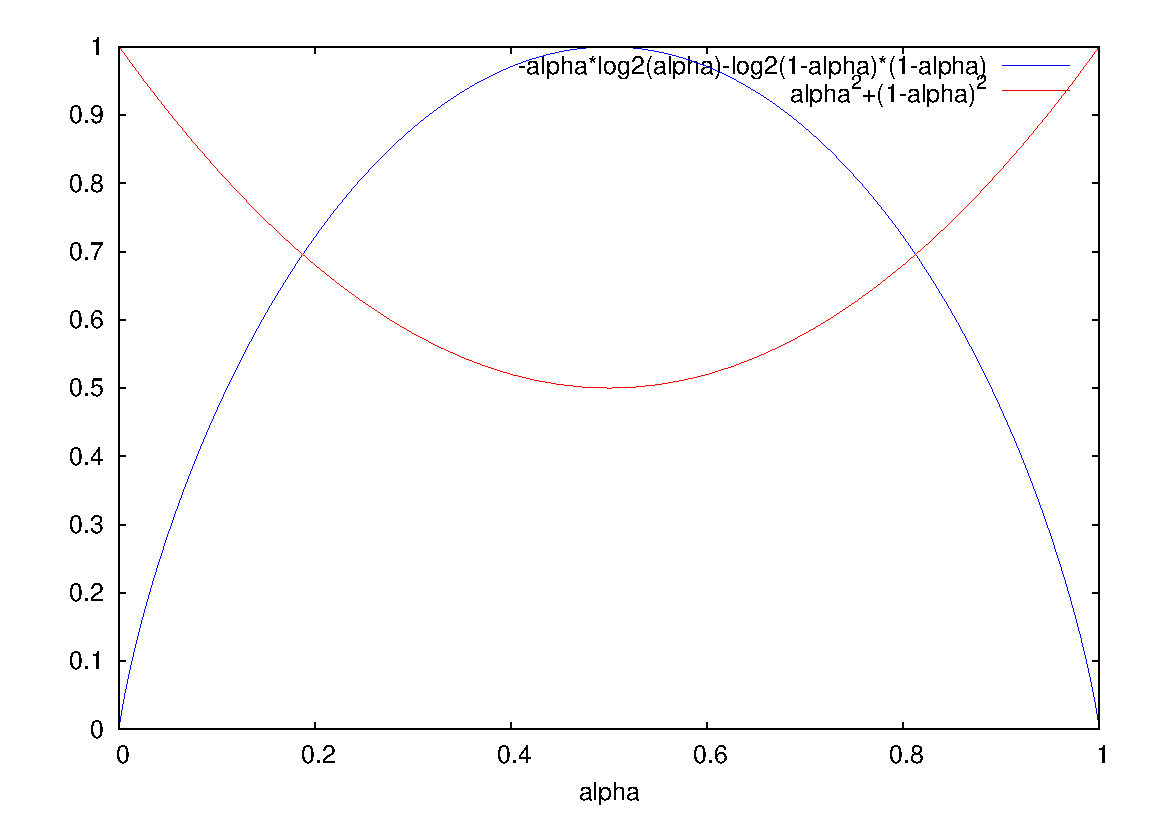
\includegraphics[width=.5\linewidth]{maxout_1.eps}
\end{dmath}

\end{document}
